\chapter{Avaliação e Resultados} \label{chap:resultados}

A hipótese levantada no âmbito desta dissertação é que o uso de abstração em imagens que vão ser ser alvo de reconhecimento facial pode melhorar o processo de reconhecimento facial automático em imagens. Para a análise desta hipótese foi criado um sistema de reconhecimento facial automático em imagens, assim  como, escolhida uma biblioteca de imagens a analisar, tal como descrito em \ref{chap:visage}. Neste capítulo, é apresentada a metodologia de avaliação adotada para a análise da hipótese levantada, assim como do sistema de reconhecimento facial Visage e são também apresentados os resultados obtidos.



-Definição da coleção base a analisar

-Definição de quais os conjuntos de teste a criar a partir da coleção base

-Definição das experiências que se pretendem realizar e porquê

-Forma de avaliar e resultados dessas experiências


\section{Conjuntos de Teste}  \label{sec:conjuntos}
O desempenho de sistemas de reconhecimento facial pode ser analisado através de diferentes perspetivas, tal como introduzido na secção \ref{sec:problema} desta dissertação. A biblioteca LFW foi criada com o propósito inicial da análise do sub-problema de reconhecimento facial \textit{pair matching}, no qual o sistema deve decidir se duas faces representam ou não o mesmo indivíduo. No entanto, as características desta biblioteca, nomeadamente no que diz respeito à existência da anotação textual das pessoas presentes em cada imagem, à existência de apenas uma pessoa representada (de forma relevante) em cada imagem e ainda da normalização do formato das imagens, permitem que esta biblioteca possa ser utilizada com um esforço reduzido para o analise dos restantes sub-problemas de reconhecimento facial automático.

No âmbito desta dissertação temos em vista a realização de um conjunto de experiências descritas em \ref{sec:experiencias} e análise dos seus resultados através de duas perspetivas descritas nos pontos \ref{sec:avaliacao1} e \ref{sec:avaliacao2} a seguir. Uma vez que estas avaliações não se encontram enquadradas no paradigma de avaliação de \textit{pair matching}, para o qual a biblioteca LFW foi originalmente criada tornou-se necessário a criação de novos conjuntos de teste.

No âmbito da avaliação de sistemas de reconhecimento facial automáticos designam-se de \textit{amostras biométricas} as capturas de características de uma pessoa que permitem efetuar o seu reconhecimento. Dependendo do sistema essas amostras biométricas podem ser apenas uma imagem, um conjunto de imagens ou um vídeo, sendo que nesta avaliação são utilizadas um conjunto de imagens. Designa-se ainda de \textit{provas} as amostras biométricas apresentadas ao sistema para serem reconhecidas.

Para a avaliação efetuada foram criados 4 conjuntos de teste. Todos os conjuntos possuem um total de 1180 imagens, correspondentes a 59 pessoas diferentes e a 20 imagens por pessoa. Dessas imagens foram criados dois conjuntos de dados: conjunto $\mathscr{G}$, designado de galeria de treino e conjunto $\mathscr{P}$, designado de provas. 

O conjunto $\mathscr{G}$ é constituído por 80\% das imagens de cada pessoa (16 imagens por pessoa), sendo as suas imagens utilizadas como amostras biométricas para o treino do sistema de reconhecimento facial. Um exemplo das imagens presentes na galeria de treino para uma pessoa pode ser visto na figura \ref{galeria}.

O conjunto $\mathscr{P}$ contem os restantes 20\% das imagens de cada pessoa (4 imagens por pessoa), e tal como o seu nome indica as suas imagens são utilizadas para a avaliação do sistema desenvolvido.

A diferença existente entre os quatro conjuntos criados encontras-se relacionada com as imagens incluídas na galeria de treino e nas provas, sendo que estas diferem de forma aleatória entre os quatro conjuntos. A criação de 4 conjuntos com igual tamanho mas diferentes imagens de treino e teste tem em vista analisar o desempenho do sistema com diferentes galerias de forma a determinar se existe uma variação significativa dos resultados obtidos em cada galeria.

\section{Experiências Realizadas} \label{sec:experiencias}
O principal objetivo desta dissertação visa a construção de um sistema de reconhecimento facial automático e o posterior estudo do impacto da utilização de filtros de abstração visual no processo de reconhecimento. O módulo de reconhecimento facial, \textit{Face Recognizer}, constituiu uma base sólida para o desenvolvimento do sistema de reconhecimento facial \textit{Visage}, contudo, de modo a tornar este sistema mais completo e versátil, revelou-se necessário adapta-lo e expandir as suas capacidades, nomeadamente através da aplicação de uma cadeia de pré-processamento às imagens existentes. Esta evolução foi feita de forma gradual e iterativa, e culminou na construção de um conjunto de galerias de imagens, analisadas através de um grupo de experiências que permitem tirar conclusões acerca dos efeitos das diversas etapas de pré-processamento realizadas e da contribuição de cada uma delas para a melhoria do desempenho do sistema criado. Todas as galerias criadas possuem as imagens contidas nos conjuntos de teste definidos em \ref{sec:conjuntos}, diferenciando-se pelos diferentes passos de pré-processamento a que as imagens foram sujeitas. Na tabela \ref{tab:colecoes} encontram-se resumidas as galerias resultantes do conjunto de experiências efetuadas, as quais se encontram descritas mais pormenorizadamente de seguida.

\subsection{Experiência 1 - Deteção e segmentação da face}
Na revisão efetuada ao estado da arte do reconhecimento facial em imagens destacou-se a importância da resolução de um conjunto de sub-problemas específicos para um reconhecimento facial eficaz, nomeadamente a deteção e segmentação das faces existentes numa imagem. Para a resolução deste problema, foi implementado o módulo de deteção facial descrito em \ref{chap:facedetector}. Na implementação deste módulo revelou-se necessário a avaliação de diferentes alternativas relativamente à forma como é efetuada a segmentação da face da restante imagem, assim como a determinação do impacto dessa segmentação. 

Após uma análise das diferente alternativas existentes, e através de alguns teste intermédios realizados durante o período de desenvolvimento, foram então criadas as galerias de imagens Original, Cropped e Masked. A primeira, é constituída pelas imagens originais da biblioteca LFW e permite estabelecer uma base de comparação entre as imagens segmentadas e as imagens originais. A galeria cropped é composta por um conjunto de imagens onde as faces foram detetadas e segmentadas pelo detetor facial implementado e descrito no capítulo \ref{chap:facedetector}. A terceira e última galeria criada possui as mesmas imagens da galeria cropped, sobre as quais foi posteriormente aplicada uma máscara elíptica de modo a diminuir a presença de fundo nas imagens recortadas.

\subsection{Experiência 2 - Normalização do Contraste}
A segunda experiência visa analisar qual a melhor forma de efetuar a normalização do contraste das imagens.

\textit{Contrast Streching}

Equalização Histograma

CLAHE


\subsection{Experiência 3 - Impacto Filtros de Abstração}
A terceira experiência visa analisar o impacto da abstração de imagens no reconhecimento.

Gaussian Blur

Bilateral

Anisotropic Kuwahara


O conjunto de imagens que constituem a biblioteca LFW-a foi ainda sujeito a um conjunto de tarefas de pré-processamento com vista a melhorar a eficácia do reconhecimento assim como analisar o impacto dos diferentes pré-processamentos na resolução do problema de reconhecimento facial automático. A cadeia de pré-processamento é constituída por quatro passos, tal como pode ser visualizado na figura \ref{fig:preprocessamento}, sendo que apenas o primeiro é obrigatório para todas as imagens pré-processadas.


\begin{center}
\begin{table}
	\caption{Sub-coleções criadas após pré-processamento.}
	\begin{center}
    \begin{tabular}{lllll}
    \hline\hline
    Designação & Recortada & Normalização           & Filtro Abstração & Máscara \\
        \hline
    Original   & -         & -                      & -                & -       \\
        \hline
    Cropped    & X         & -                      & -                & -       \\
    Masked     & X         & -                      & -                & X       \\
        \hline
    Normalized & X         & Constrast Streching    & -                & X       \\
    Equalized  & X         & Histogram Equalization & -                & X       \\
    CLAHE      & X         & CLAHE                  & -                & X       \\
        \hline
    Bilateral  & X         & Histogram Equalization & Bilateral Filter & X       \\
    Gaussian   & X         & Histogram Equalization & Gaussian Filter  & X       \\
    \hline\hline
    \end{tabular}
	\label{tab:colecoes}
	\end{center}
\end{table}
\end{center}

Da aplicação de diferentes combinações de pré-processamentos aplicados sobre as imagens da coleção LFW-a resultou a criação de um conjunto de novas coleções,  tal como pode ser visualizado na tabela \ref{tab:colecoes}. O primeiro conjunto desta tabela corresponde à coleção original, sobre a qual não foram aplicadas quaisquer tarefas de pré-processamento. Os conjuntos \textit{Masked} e \textit{Cropped}, têm em vista analisar o impacto da remoção de informação redundante que se encontra na imagem, devido à existencia de uma grande àrea de fundo, onde existem, por exemplo, faces de outras pessoas na coleção original. OS conju


\section{Resultados}
Os conjuntos de testes descritos em \ref{sec:conjuntos} foram avaliados em cada uma das experiências descritas em \ref{sec:experiencias}. Para cada conjunto, quando uma prova $p_j$ é apresentada ao sistema, essa prova é então comparada a cada amostra biométrica $g_i$ da galeria, resultando dessa comparação o respetivo índice de similaridade (\textit{similarity score}), $s_{ij}$. Este índice é designado de $match$ $score$, caso $g_i$ e $p_j$ sejam amostras da mesma pessoa, caso não o sejam é designado de $nonmatch$ $score$. Quanto menor o índice de similaridade, maior é a probabilidade das imagens comparadas pertencerem à mesma pessoa, sendo que o melhor valor possível para o índice de similaridade de um $match$ $score$ é zero.

A qualidade do desempenho de um sistema de reconhecimento facial automático, assim como a satisfação dos seus utilizadores está intimamente relacionada com o fim para o qual o sistema foi criado. No âmbito desta dissertação, a avaliação do desempenho foi efetuada segundo duas perspetivas distintas, \textit{Closed-set Identification} e \textit{Image Retrieval}, as quais são apresentadas de seguida.

\subsection{Resultados \textit{Closed-Set Identification}} \label{sec:avaliacao1}
Tal como introduzido na secção \ref{sec:problema}, o paradigma de \textit{closed-set identification}, constitui um sub-problema de identificação em que uma prova é apresentada ao sistema e pretende-se que este devolva a identidade da pessoa presente na imagem. Neste caso particular do problema de identificação, todas as provas apresentadas possuem uma correspondência na galeria, em oposição ao caso geral de identificação em que pode ou não haver uma correspondência.

A avaliação \textit{closed-set} é uma medida padrão de avaliação do desempenho em sistemas de reconhecimento facial automático, tendo sido utilizada em diversas avaliações efetuadas, nomeadamente nas avaliações FERET e FRVT apresentadas na revisão do estado da arte desta dissertação (ver \ref{chap:reco}). A utilização de um conjunto fechado de imagens permite uma análise mais detalhada do desempenho de um algoritmo permitindo responder à pergunta "a identificação correta encontra-se nos primeiros $n$ resultados?" em vez de apenas " o primeiro resultado é o correto?".

\subsubsection{Metodologia Avaliação}
Seja $p_j$, uma prova do conjunto de provas $\mathscr{P}$. Na identificação de $p_j$, em primeiro lugar são calculados os índices de similaridade para todas as amostras na galeria $\mathscr{G}$, sendo posteriormente ordenados os seus resultados. Uma prova $p_j$ tem ranking $n$ se o seu $match$ $score$ corresponde ao enésimo menor índice de similaridade. A taxa de identificação para o ranking $n$, $T_{I}(n)$, corresponde à fração de provas com ranking $n$ ou menor do que $n$, ou seja:
\begin{equation}
T_{I}(n) = \frac{|C(n)|}{|\mathscr{P}|} \times 100
\end{equation}
Em que $|C(n)|$ é número de provas com ranking $n$, ou menor do que $n$, e $|\mathscr{P}|$ o número de provas existentes em $\mathscr{P}$.
 
Os resultados da identificação são posteriormente representados num gráfico do tipo \textit{Cumulative match score} (CMS). Um gráfico do tipo CMS representa $T_{I}(n)$ como uma função de ranking $n$. No eixo horizontal encontra-se representado o ranking e no eixo vertical encontra-se representada a respetiva taxa de identificação.

\subsubsection{Resultados Experiência 1}

\begin{figure}[h]
        \centering
        \begin{subfigure}[b]{0.65\textwidth}
                \centering
                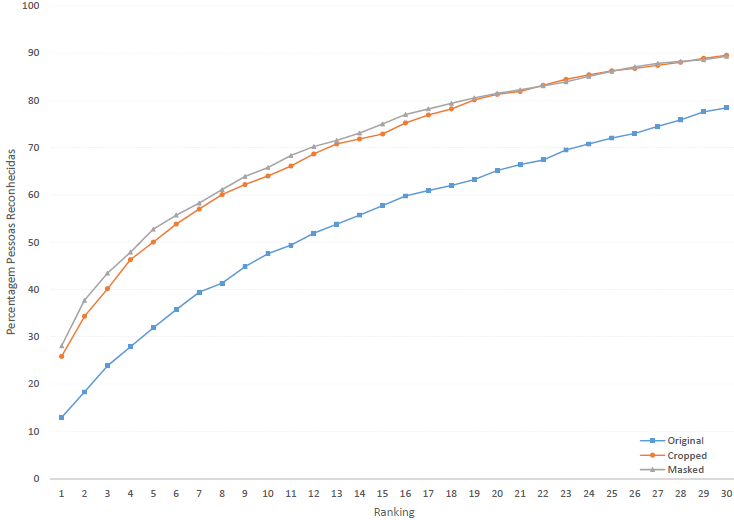
\includegraphics[width=\textwidth]{resultados/original_cropped_masked_eigen}
                \caption{Eigenfaces}
                \label{fig:original_cropped_masked_eigen}
        \end{subfigure}%
        
        ~ %add desired spacing between images, e. g. ~, \quad, \qquad etc.
          %(or a blank line to force the subfigure onto a new line)
        \begin{subfigure}[b]{0.65\textwidth}
                \centering
                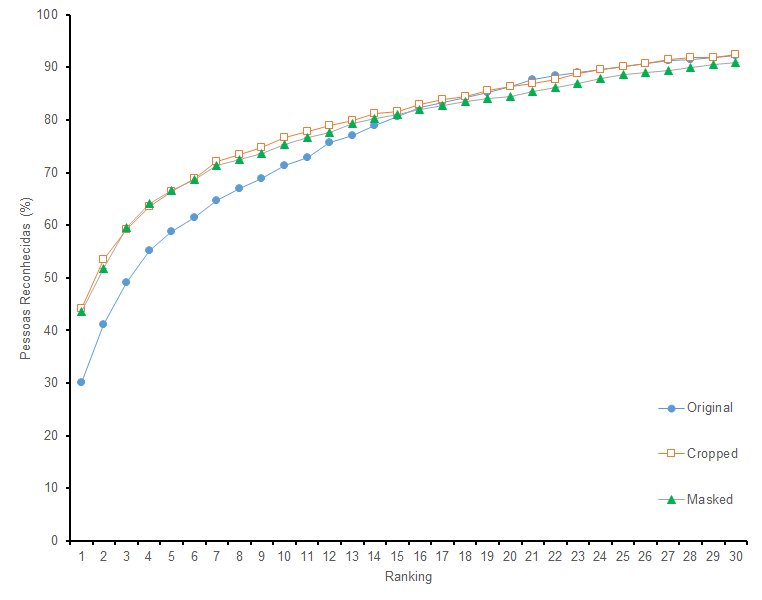
\includegraphics[width=\textwidth]{resultados/original_cropped_masked_fisher}
                \caption{Fisherfaces}
                \label{fig:original_cropped_masked_fisher}
        \end{subfigure}
        
        ~ %add desired spacing between images, e. g. ~, \quad, \qquad etc.
          %(or a blank line to force the subfigure onto a new line)
        \begin{subfigure}[b]{0.65\textwidth}
                \centering
                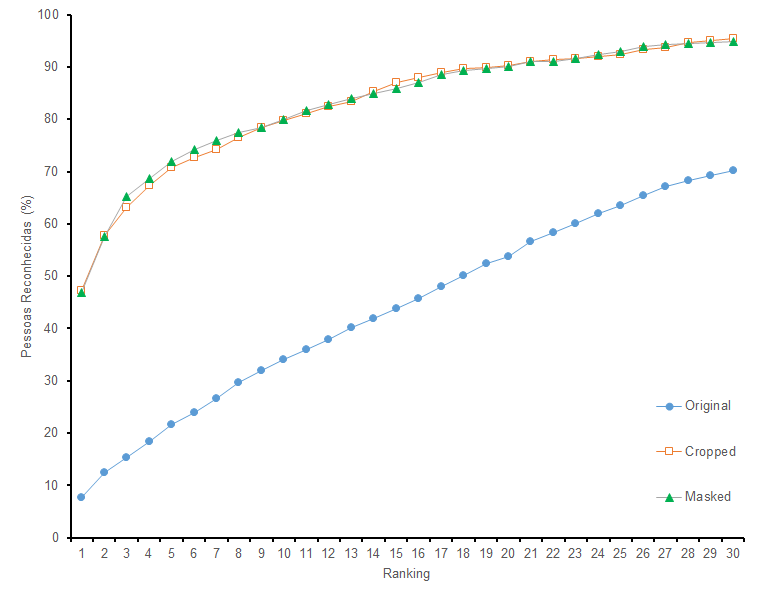
\includegraphics[width=\textwidth]{resultados/original_cropped_masked_lbph}
                \caption{LBPH}
                \label{fig:original_cropped_masked_lbph}
        \end{subfigure}
        \caption{Desempenho algoritmos Eigenfaces, Fisherfaces e LBPH para os conjuntos Original, Cropped e Masked}\label{fig:original_cropped_masked}
\end{figure}

Esta experiência visa analisar o impacto da segmentação das faces presentes na imagem do fundo existente nas mesmas, assim como determinar qual, de entre duas alternativas, a melhor forma de segmentar essa mesma face. Os resultados obtidos podem ser visualizados na figura \ref{fig:original_cropped_masked}, onde se encontram ilustrada a performance dos algoritmos de teste, \textit{Eigenfaces}, \textit{Fisherfaces} e \textit{LBPH}, nos três conjuntos criados especialmente para esta experiência, original, cropped e masked, os quais se encontram descritos mais pormenorizadamente em \ref{sec:experiencias}.

Após a analise dos resultados obtidos na experiência 1 verifica-se que a segmentação das faces presentes nas imagens originais produz uma melhoria efetiva dos resultados obtidos, traduzindo-se num aumento de cerca de 12\%, 14\% e 40\% para a taxa de identificação de ranking 1 dos algoritmos \textit{Eigenfaces}, \textit{Fisherfaces} e \textit{LBPH}, respetivamente.

Uma análise mais aprofundada desses resultados, demonstra ainda que, no caso dos algoritmos \textit{Eigenfaces} e \textit{LBPH}, a diferença na taxa de identificação entre as imagens originais e as imagens segmentadas é significativa e relativamente constante nos vários níveis para os quais a taxa de deteção se encontra reportada. Por outro lado, no caso do algoritmo \textit{Fisherfaces}, apesar da diferença significativa no número de imagens corretamente identificadas nos primeiros níveis, a partir do ranking 15, todos os conjuntos de imagens obtém uma taxa de identificação similar, e com uma progressão semelhante. Esta aproximação no número de caras corretamente identificadas nos rankings mais elevados pode ser explicada pela existência de informação no fundo das imagens, a qual poderá ser utilizada pelo próprio algoritmo para a identificação das mesmas, ao invés da utilização da face contida na imagem, reforçando assim a importância da extração do fundo contido nas imagens originais.

Por outro lado, note-se ainda que, apesar do impacto positivo da segmentação das imagens nos três algoritmos testados, o impacto desta segmentação varia significativamente conforme o algoritmo utilizado, sendo que o \textit{Fisherfaces} é o que revela resultados mais constantes independentemente da manipulação efetuada nas imagens e o algoritmo \textit{LBPH} o que regista uma maior melhoria desses mesmos resultados.

Ao nível da diferença entre as imagens apenas segmentadas (conjunto Cropped) e as imagens com máscara (conjunto Masked), é possível verificar que ambas possuem resultados semelhantes, sendo que a maior diferença foi detetada no algoritmo \textit{Eigenfaces}, onde as imagens com máscara demonstraram um desempenho ligeiramente superior, como é possível verificar pelas $T_{I}(2)$ de 43,4\% e 40,1\% para as imagens com máscara e recortadas, respetivamente. A existência de uma máscara garante, no entanto, uma extração de uma maior quantidade de fundo das imagens, permitindo assim uma maior confiança dos resultados obtidos no sentido em que se reduz o perigo de identificação pelas características do próprio fundo e não das caraterísticas faciais presentes na imagem. 

Finalmente, ao nível dos algoritmos utilizados é possível verificar que o algoritmo \textit{LBPH} obtém resultados globalmente melhores nos conjuntos segmentados, ao passo que o algoritmo \textit{Eingefaces} obtém os piores resultados. Esta diferença verifica-se quer nos rankings mais inferiores, quer nos superiores, sendo menor quanto maior é o ranking utilizado, como é possível verificar pelas taxas de identificação de ranking 1 de 46,8\% e 28,1\%, no conjunto Masked, para os algoritmos \textit{LBPH} e \textit{Eigenfaces}, respectivamente e pelas taxas de identificação de ranking 30 de 94,9\% e 89,3\%, para o mesmo conjunto.

\subsubsection{Resultados Experiência 2}

\subsubsection{Resultados Experiência 3}


\subsection{Resultados em Retrieval} \label{sec:avaliacao2}
Criação de um sistema de reconhecimento facial automático com vista à aplicação em image retrieval

\subsubsection{Metodologias Avaliação}

\subsubsection{Resultados}

